% Three spike encoding schemes
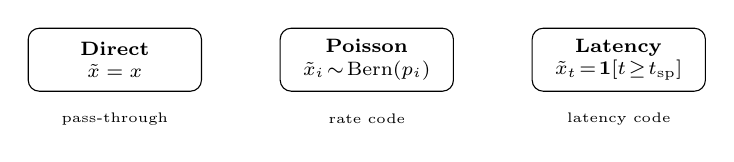
\begin{tikzpicture}[font=\scriptsize, >=latex, every node/.style={align=center}]
  \node[draw, rounded corners, minimum width=22mm, minimum height=8mm] (d1)
    at (-3.2, 0) {\textbf{Direct}\\$\tilde{x}=x$};
  \node[draw, rounded corners, minimum width=22mm, minimum height=8mm] (d2)
    at (0, 0) {\textbf{Poisson}\\$\tilde{x}_i\!\sim\!\mathrm{Bern}(p_i)$};
  \node[draw, rounded corners, minimum width=22mm, minimum height=8mm] (d3)
    at (3.2, 0) {\textbf{Latency}\\$\tilde{x}_t\!=\!\mathbf{1}[t\!\geq\!t_{\mathrm{sp}}]$};
  \node[font=\tiny] at (-3.2,-0.75) {pass-through};
  \node[font=\tiny] at (0,-0.75) {rate code};
  \node[font=\tiny] at (3.2,-0.75) {latency code};
\end{tikzpicture}
